% 6.8 -- converted from manuscript.md lines 597-709 (source of truth).
\subsection{Prediction-anchored Poisson count, and its mass generalization}\label{sec:count}

Every verdict so far is anchored operationally: a margin taken from an
exploration block, or a threshold declared before sizing. This stage is
different. The diamond-volume oracle certifies an interval for the continuum
4-volume $V$ of a fixed causal diamond, by directed-rounding arithmetic and
before any count data exists; a Poisson sprinkling then supplies a count of
elements certified to lie inside that same diamond. The question is whether
the operational instrument realizes the certified prediction. Nothing in
sections~\ref{sec:capstone}--\ref{sec:schwarzschild} is used to answer it,
and the answer cannot be tuned after the fact: the endpoints, the intensity,
the tolerance and the decision rule are all frozen in the rung's
preregistration before its seed is drawn. The stage also closes a loop the
flat ladder left open: rung R1 consumed a supplied density to convert counts
into volumes, validated there against targets the same machinery produced;
here that same count-to-volume conversion---the number-volume correspondence
at the root of the causal-set program~\cite{sorkin1997forks}---is
confronted, on a Schwarzschild diamond, with a volume certified
independently of it.

\textbf{The instrument.} Points are sprinkled at a frozen intensity $A$ into
the certified box, and each point's membership is decided by the certified
causal predicate on both legs. A point the predicate cannot decide at the
frozen tolerance is \emph{not guessed}: it is counted as ambiguous
($U_{\mathrm{amb}}$) and enters the decision only through the conservative
end of the interval. Each rung first runs a fixed-$n$ ambiguity pilot (exact
Clopper--Pearson plus an exact Poisson tail bound at $\alpha = 0.01$, tail
budget $1\times10^{-3}$) that must certify $U_{\mathrm{max}} \le 30$ before
the count campaign is sized; the campaign's membership test short-circuits
on a decided first leg, so a point the campaign calls ambiguous is
necessarily one the pilot's test would also call ambiguous, and the pilot's
bound transfers \emph{a fortiori}.

\textbf{The frozen rule.} From the realized
$(K_{\mathrm{certain}}, U_{\mathrm{amb}})$ the rule builds a deliberately
conservative \emph{outer} count interval---the exact
Garwood~\cite{garwood1936} lower limit at
$K_{\mathrm{certain}}$, the upper limit at
$K_{\mathrm{certain}} + U_{\mathrm{amb}}$, each tail at level 0.025, so the
ambiguous points can only widen the interval outward and never move it
toward agreement. Rescaled by the intensity this is a volume interval
$C = [L/A, U/A]$, and the quantity gated is the \emph{identified
discrepancy} against the certified enclosure,
\begin{equation}
\begin{array}{c}
D = [C_{\mathrm{lo}} - V_{\mathrm{hi}},\; C_{\mathrm{hi}} - V_{\mathrm{lo}}],
\quad \mbox{required to lie in } [-B, +B],\\[2pt]
B = \tau V_{\mathrm{ref}}, \quad \tau = 2.5\%,
\end{array}
\end{equation}
with three ways out and no fourth: contained gives CONCORDANT, disjoint
gives DISCORDANT, and anything else gives INCONCLUSIVE, published as it
falls. The arithmetic is 96-bit end to end, and contract tests prove at the
integer boundaries that the frozen acceptance window is exactly the set of
counts the decision function calls CONCORDANT, so ``the sizing'' and ``the
verdict'' cannot drift apart. The gate is a confidence-interval form of
the two one-sided tests procedure~\cite{schuirmann1987,lakens2017} on exact
intervals, in the model-validation sense of requiring a discrepancy to fall
inside a pre-set band~\cite{robinsonfroese2004}; its statistical novelty is
the preregistered application against a certified enclosure, not the
apparatus.

\textbf{The ladder.} One rung would establish the gate at one geometry. To
ask whether the agreement is a property of the instrument rather than of a
lucky configuration, the same gate is carried across a preregistered mass
ladder. The certified shell $[10, 20]$ and the anchors $(12, 18)$ stay
fixed in \emph{absolute} coordinates, so no rung
is an isometric copy of another: the pre-frozen dimensionless indicator is
the compactness $\mu = 2M/r_c$ at the anchor midpoint $r_c = 15$, and the
executed ladder spans a factor of three in it. The mass is not the only thing
that moves, and the second motion narrows what the ladder can show. The
diamond's coordinate-time window is retuned per rung by the
frozen rule $dt(M) = 8.5\,T_{\mathrm{min}}(M)/T_{\mathrm{min}}(1)$, so that
each rung opens the same multiple of its own minimal flight time; the whole
diamond therefore scales with that flight time. The consequence is worth
stating plainly: the certified
volumes track $(dt/dt_1)^2$ to 0.007\%, 0.021\% and 0.144\% at $M = 1.4$, 1.8
and 3.0, so their mass-specific content sits one to two orders of magnitude
below the $\tau = 2.5\%$ band the gate applies. The deep end is not a free
choice either: every mass-generic lemma certifies exactly on
$M \in [0.92, 3.33]$---bounded above by the photon sphere $3M$ reaching the
shell floor at $M = 10/3$---and the deepest rung $M = 3.0$ keeps a certified
margin of a tenth of the shell floor on that binding condition---by
certification rather than by taste---its inner
anchor at $r = 4M$ between the photon sphere and the ISCO. The patch-level
lemmas are mass-generic only under stated conditions (horizon below the
shell, $K < 0$, $w$ monotone, $Q > 0$, the L2a patch bound, four L4 margins,
an L5 winding cross-check), and each is re-certified per rung as an interval
comparison---nothing is inherited silently from $M = 1$.

Four rungs were executed, each from its own exact freeze checkout, with its
own seed, once (\tref{tab:count}).

\begin{table}[t]
\caption{The four executed mass-ladder rungs: certified volume interval
$V$, pilot ambiguity outcome, sprinkled $N$, certain and ambiguous counts,
outer count interval $C$, identified discrepancy $D$, band $B$, and
verdict.}
\label{tab:count}
\centering
\scriptsize
\setlength{\tabcolsep}{2.5pt}
% Each rung occupies two physical rows: the three interval columns
% (certified V, C, D) carry their lower endpoint on the first row and
% their upper endpoint on the second, so the table fits the text width
% without shrinking below \scriptsize.
\begin{tabular}{@{}ccccccccccc@{}}
\toprule
$\mu$ & $M$ & certified $V$ & pilot & $N$ & $K_{\mathrm{certain}}$ & $U_{\mathrm{amb}}$ & $C$ & $D$ & $B$ & verdict \\
\midrule
$0.1333$ & $1.0$ & $[56.492959,$ & $k=0$ & 26,831,117 & 53,285 & 0 & $[56.205871,$ & $[-0.854796,$ & $1.419420$ & \textbf{CONCORDANT} \\
 & & $\phantom{[}57.060667]$ & & & & & $\phantom{[}57.169553]$ & $\phantom{[}{+}0.676594]$ & & \\
\addlinespace
$0.1867$ & $1.4$ & $[64.336198,$ & $k=1$ & 15,057,284 & 53,829 & 1 & $[64.307488,$ & $[-0.675256,$ & $1.616487$ & \textbf{CONCORDANT} \\
 & & $\phantom{[}64.982744]$ & & & & & $\phantom{[}65.405648]$ & $\phantom{[}{+}1.069450]$ & & \\
\addlinespace
$0.2400$ & $1.8$ & $[73.968637,$ & $k=0$ & 9,847,124 & 53,513 & 0 & $[73.695211,$ & $[-1.016709,$ & $1.858507$ & \textbf{CONCORDANT} \\
 & & $\phantom{[}74.711920]$ & & & & & $\phantom{[}74.956037]$ & $\phantom{[}{+}0.987400]$ & & \\
\addlinespace
$0.4000$ & $3.0$ & $[121.225021,$ & $k=0$ & 4,605,671 & 53,606 & 0 & $[120.802632,$ & $[-1.640649,$ & $3.045854$ & \textbf{CONCORDANT} \\
 & & $\phantom{[}122.443280]$ & & & & & $\phantom{[}122.867592]$ & $\phantom{[}{+}1.642571]$ & & \\
\bottomrule
\end{tabular}
\end{table}

\begin{figure}[t]
\centering
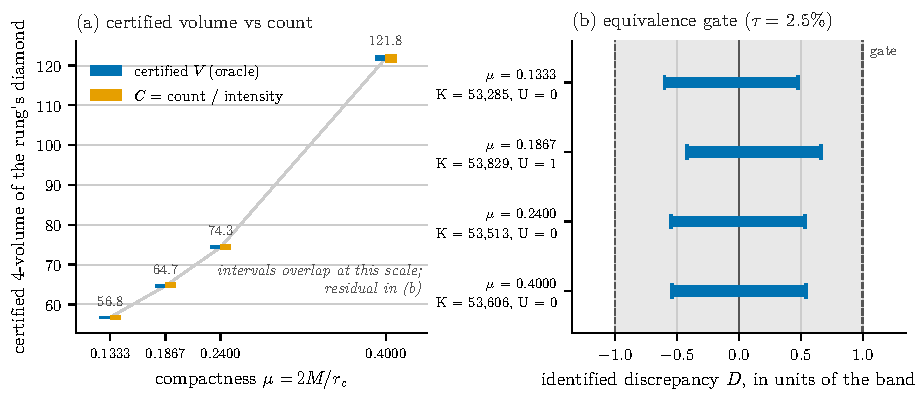
\includegraphics[width=\textwidth]{figures/fig6_ladder_count.pdf}
\caption{The executed ladder. (a)~At each preregistered compactness, the
certified continuum volume (blue) and the volume implied by the sprinkled
count (orange). The intervals overlap at plot scale across a threefold span
in $\mu$---that overlap, at each rung independently, is the result; the
cross-rung span is not itself a curvature signal (\sref{sec:count}).
(b)~The residual made visible: each
rung's identified discrepancy $D$ divided by that rung's own band
$B = \tau V_{\mathrm{ref}}$, so the rungs are comparable despite different
bands; the shaded region is the gate. Every rung is contained, with roughly
half the band to spare, and the $\mu = 0.1867$ rung's asymmetry is its
single ambiguous point widening the interval outward as the rule provides.
Both panels are generated from the same artifacts the contract tests
re-derive (\artifact{latex/\allowbreak{}figures/\allowbreak{}make\_\allowbreak{}journal\_\allowbreak{}figures.py}, reading the same artifacts as the manuscript's \artifact{figures/\allowbreak{}make\_\allowbreak{}ladder\_\allowbreak{}figure.py}); no value is typed
in.}
\label{fig:count}
\end{figure}

The certified volume grows monotonically with the compactness (57 to 65 to
74 to 122), and the realized discrepancy
stays well inside the band at every rung (\fref{fig:count}). The $M = 1.4$
pilot
returned the program's first non-zero ambiguous count ($k = 1$); it was
absorbed exactly as the sizing had provisioned, and it is visible in that
rung's asymmetric $D$, which is the conservative widening working as
designed rather than a defect.

\textbf{What this establishes.} On each preregistered rung independently, an
operational finite-density instrument realized that rung's independently
certified continuum volume to within $\tau = 2.5\%$, under a rule fixed
before the data existed. This is the first place in the program where a
measurement is confronted with a certified \emph{prediction} rather than
with an operational anchor, and the confrontation is repeated at four masses
rather than one---the deepest with its inner anchor between the photon sphere
and the ISCO. What the repetition buys is not four independent curvature
probes---the volumes are near-degenerate across rungs, as stated
above---but the re-certification of every patch-level lemma and a fresh run
of the causal predicate at each mass, none of it inherited from $M = 1$.

\textbf{What it does not establish.} The rungs are separate preregistered
stages: each verdict stands alone, there is no joint primary verdict, and no
interpolation, extrapolation, or composite cross-rung statistic is
claimed---in particular nothing is claimed at compactness between or beyond
the four tested values. Agreement of a count with a volume is not a test of
causal-set theory, and it is not evidence that spacetime is discrete; it is
a statement that this instrument, at these operating points, reproduces the
continuum measure it was pointed at. It upgrades neither the C1/C2 verdicts
of sections~\ref{sec:capstone}--\ref{sec:schwarzschild} nor the auxiliary
O4b instrument audit, none of which use it. And the result is bounded by its
construction exactly as the capstone is: one fixed diamond, one fixed
density per rung, a Schwarzschild exterior shell, and a tolerance chosen to
be feasible rather than to be sharp.
